\documentclass{article}
\usepackage[a4paper]{geometry}
\usepackage{asymptote,comment}
\usepackage{pgfplots}
\pgfplotsset{compat=1.18}
\begin{document}

Jaglal, Tyler - Math 115, AS01 - Investigation into Intersecting Cylinders
\hrule

\vspace{10pt}

This topic was originally discussed in the LaTeX development community two years ago in this post: https://tex.stackexchange.com/questions/404273/how-to-draw-two-intersecting-cylinders?noredirect=1\&lq=1

\vspace{10pt}

I fiddled around with the code from the above link lasst night and was able to implement a third cylinder. In doing so, I have developed a confidence that I could create similar diagrams.

\begin{center}
\begin{tikzpicture}[scale=3]
  \begin{axis}[%
        axis equal,
        enlargelimits = true,
        samples = 45, samples y = 45,
        axis lines = none, ticks = none,
        cyl/.style = {%
                surf,
                black!30!,
                variable = \u,
                variable y = \v,
                z buffer = sort,
                faceted color=black!70!,
                },
        %view/h = 125, view/v = 25
        ]

    \addplot3[%         (-) Z-SEMIAXIS
        cyl,
        domain = -3:3,
        y domain = 0:360,
        ] ({cos(v)}, {sin(v)}, {min(u,abs(cos(v)),abs(sin(v)))});

    \addplot3[%         (-) X-SEMIAXIS
        cyl,
        domain = -3:3,
        y domain = 0:360,
        ] ({min(u,-abs(cos(v)),-abs(sin(v)))}, {cos(v)}, {sin(v)});


    \addplot3[%         (+) Y-SEMIAXIS
        cyl,
        domain = 0:360,
        y domain = -3:3,
        ] ({cos(u)}, {max(v,abs(cos(u)),abs(sin(u)))}, {sin(u)});

    \addplot3[%         (+) X-SEMIAXIS
        cyl,
        domain = -3:3,
        y domain = 0:360,
        ] ({max(u,abs(cos(v)),abs(sin(v)))}, {cos(v)}, {sin(v)});

    \addplot3[%         (+) X-SEMIAXIS
        cyl,
        domain = -3:3,
        y domain = 0:360,
        ] ({cos(v)}, {sin(v)}, {max(u,abs(cos(v)),abs(sin(v)))});

    \addplot3[%         (-) Y-SEMIAXIS
        cyl,
        domain = 0:360,
        y domain = -3:3,
        ] ({cos(u)}, {min(-abs(cos(u)),-abs(sin(u)),v)}, {sin(u)});

    \end{axis}
\end{tikzpicture}
\end{center}

\vspace{10pt}

I am still having trouble completing the parametric function for a portion off  the surface of intersection of the cylinders; this is what I've got so far, and a link to an active discuss I am having on the topic is in the email

\begin{center}
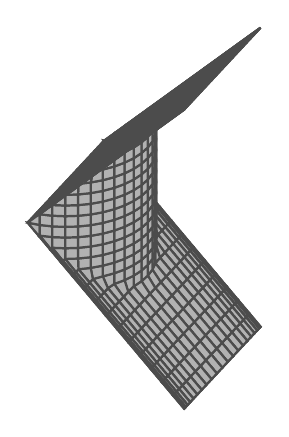
\begin{tikzpicture}[scale=2]
  \begin{axis}[%
        axis equal,
        enlargelimits = true,
        samples = 45, samples y = 45,
        axis lines = none, ticks = none,
        cyl/.style = {%
                surf,
                black!30!,
                variable = \u,
                variable y = \v,
                z buffer = sort,
                faceted color=black!70!,
                },
        %view/h = 125, view/v = 25
        ]

    \addplot3[%         (-) Z-SEMIAXIS
        cyl,
        domain = -3:3,
        y domain = 0:360,
	  restrict z to domain=-2:2,
        ] ({max(abs(u),cos(v))}, {sin(v)}, {u});

    \end{axis}
\end{tikzpicture}
\end{center}

\newpage

And this is a solution using Asymptote; when I learn Asymptote, I am confident that I could do it in a more visually appealing way:
\begin{comment}
\begin{center}
\begin{asy}
  import graph3;
  import solids;

  size(0,150);
  currentprojection=orthographic(1,1/2,1/2);

  // usage revolution r = cylinder(start,radius,length,ax);
  revolution r=cylinder(O,1,8,X);
  draw(surface(r),gray,render(merge=true));
  revolution r=cylinder((4,-4,0),1,8,Y);
  draw(surface(r),gray(0.8),render(merge=true));
 \end{asy}

 \begin{asy}
  import graph3;
  import solids;

  size(0,150);
  currentprojection=orthographic(1,1/2,1/2);

  // usage revolution r = cylinder(start,radius,length,ax);
  revolution r=cylinder(O,1,8,X);
  draw(surface(r),gray,render(merge=true));
  revolution r=cylinder((4,0,0),1,4,Y);
  draw(surface(r),gray(0.8),render(merge=true));
  draw((3.5,-1,1) -- (0,-1,1),  arrow=Arrow3(TeXHead2));
  draw((4.5,-1,1) -- (8,-1,1),  arrow=Arrow3(TeXHead2));
  label("$L_1$",(4,-1,1));
 \end{asy}
\end{center}
\end{comment}
\end{document}